\documentclass[10pt,a4paper,twoside]{article}
\usepackage[dutch]{babel}
%laad de pakketten nodig om wiskunde weer te geven :
\usepackage{amsmath,amssymb,amsfonts,textcomp}
%laad de pakketten voor figuren :
\usepackage{graphicx}
\usepackage{float,flafter}
\usepackage{hyperref}
\usepackage{inputenc}
%zet de bladspiegel :
\setlength\paperwidth{20.999cm}\setlength\paperheight{29.699cm}\setlength\voffset{-1in}\setlength\hoffset{-1in}\setlength\topmargin{1.499cm}\setlength\headheight{12pt}\setlength\headsep{0cm}\setlength\footskip{1.131cm}\setlength\textheight{25cm}\setlength\oddsidemargin{2.499cm}\setlength\textwidth{15.999cm}

\begin{document}
\begin{center}
\hrule

\vspace{.4cm}
{\bf {\Huge Problem 4}}
\vspace{.2cm}
\end{center}
{\bf Name: Cheng Chen}  \\
{\bf ID:40222770}\\
{\bf function: tan(x)}\\
{\bf Concordia University}\\
SOEN 6011: Software Engineering Processes {\bf  } \hspace{\fill}  17 July  2022 \\
\hrule
%\bf genereert vette letters, \large \Large \huge \Huge \tiny \small ... verschillende lettergroottes, met \em, \it, \sl krijg je cursieve tekst
%Je moet accolades gebruiken om aan te geven waarop je het commando precies wil laten inwerken.
% commentaar zet je in de tex-file met een %-tekentje voor.



%de ~ zorgt ervoor dat het ! met een spatie aan de tekst wordt geplakt en niet naar de volgende lijn verhuist.  Omdat latex na elk . automatisch een dubbele spatie invoegt, kan je ~ ook gebruiken om te voorkomen dat je na een afkorting bvb.~een dubbele spatie krijgt.

%1 open lijn wordt door latex gewoon als spatie gezien, met twee linefeeds  begint een nieuwe paragraaf.  Als je wil voorkomen dat de tekst inspringt, kan je het commando \noindent gebruiken.  \\ springt naar een volgende lijn, \newpage naar een volgend blad.


%\begin{figure}
%\centering
%\includegraphics[width=0.7\linewidth]{figje}
%\caption{}
%\label{fig:figje}
%\end{figure}
\section{Description}
tan1.java and tan2.java are based on Code Conventions for the Java TM Programming Language.\cite{ref1}
\subsection{Mindmap for Java style}
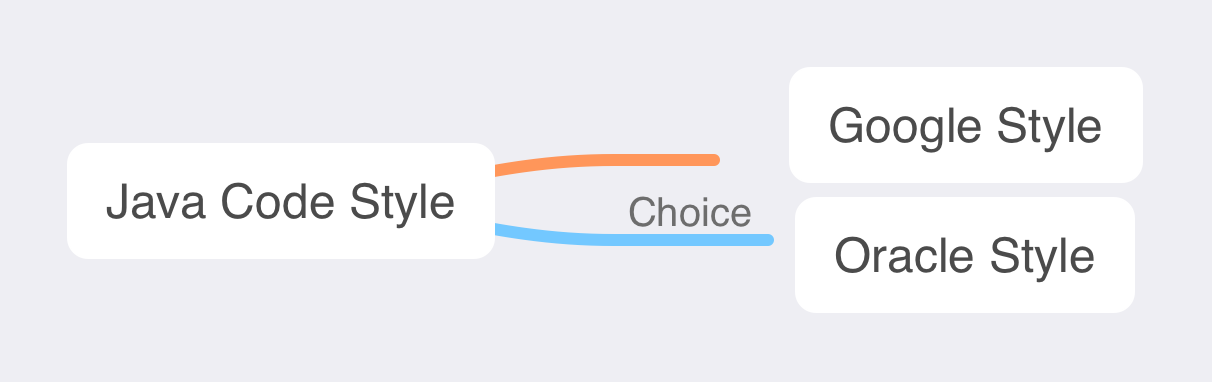
\includegraphics[scale=0.60]{javacodestyle.png}

\subsection{error handling}
    Both tan1.jar and tan2.jar offer error handling. If the user type something that is not a single real number, both programs will return the message "Please input numbers only!"
\subsection{Debugger}
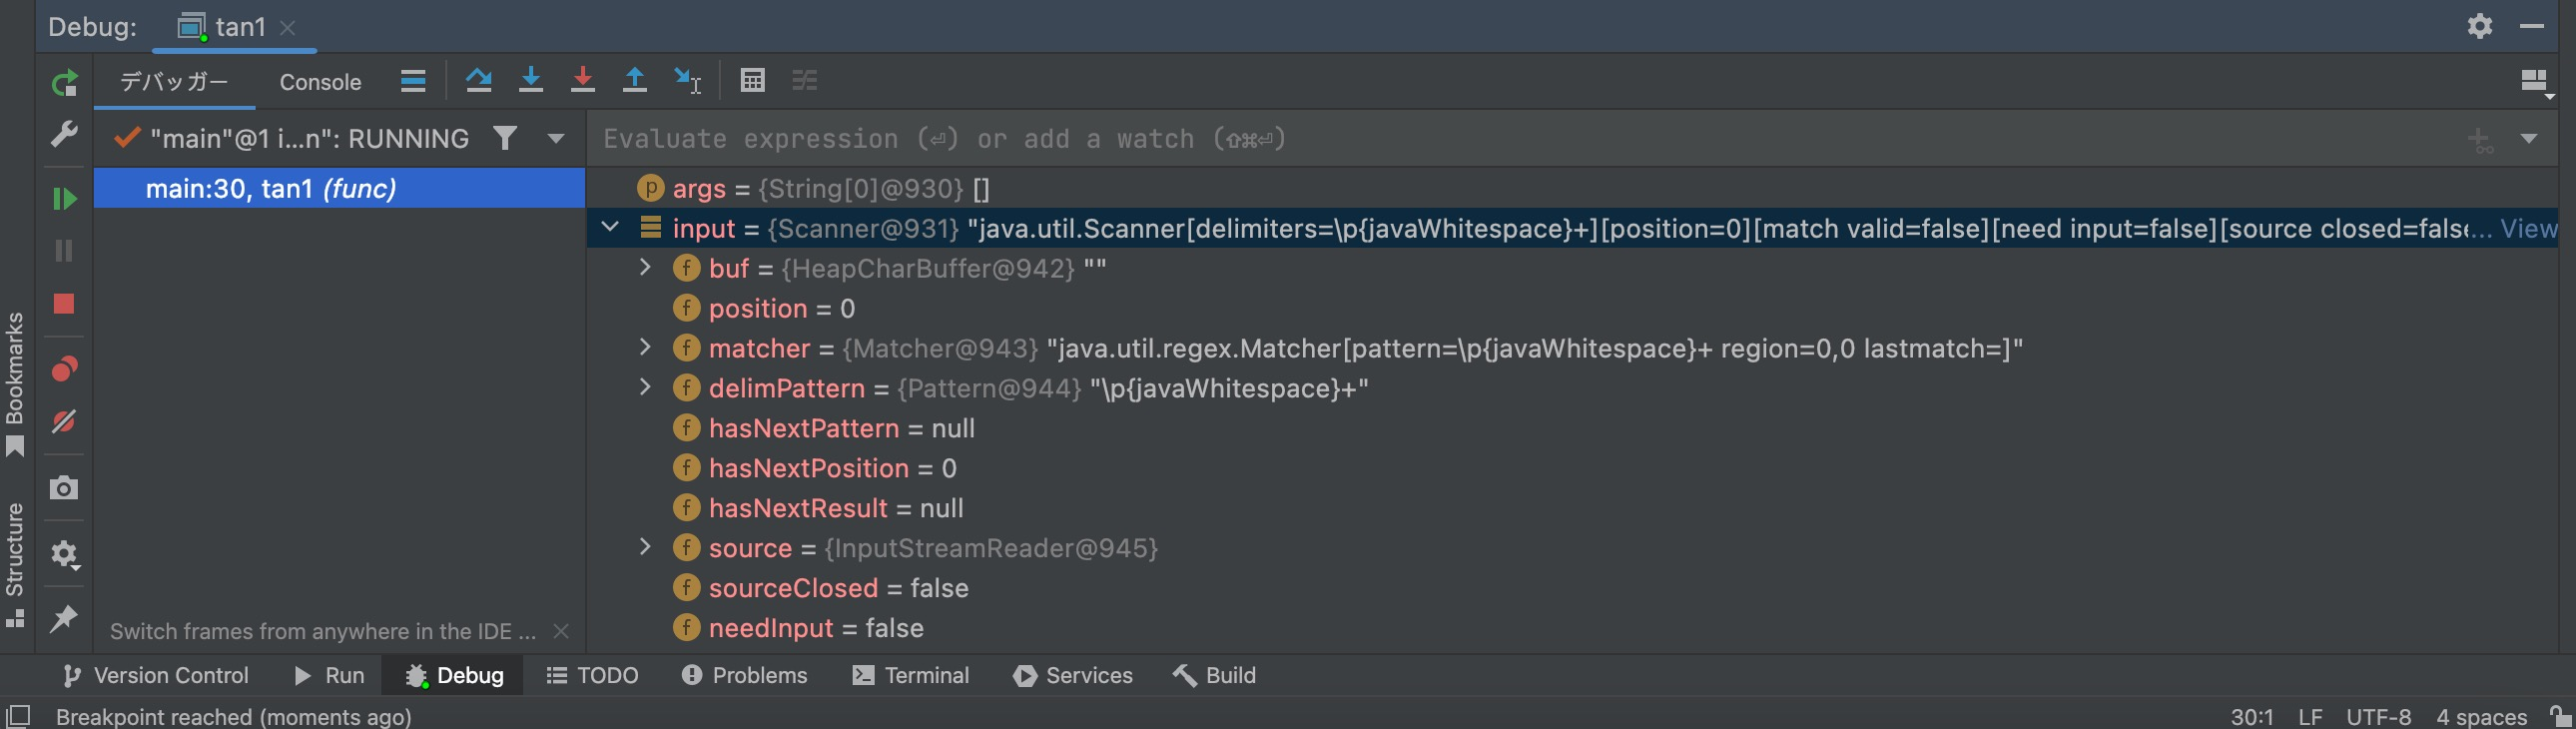
\includegraphics[scale=0.15]{debugger.png}
\begin{itemize}
    \item advantages:by setting breakpoints at any statement where the user wants to set, the debugger(デバッガー in the picture means debugger :https://www.linguee.com/japanese-english/translation/デバッガー.html) help the user identify the status of the variables, and continue the program sentence by sentence to observe the change of the variables.
    
    \item disadvantages: not new users friendly. The user needs to set breakpoints to use the debugger completely. No response if there is no breakpoint, there should be information telling the user to set.
    Besides, the debugger is hard to help if the execution is stopped inside an invariant.
\end{itemize}


\subsection{code characteristics}
correct:99 percent accuracy.
robust:check if the input is right.
time-efficient:use a hard-coded formula.
usable:can compute tan(x) with 0.01
%Met het commando \sectie{naamtitel} maak je een nieuwe titel aan.
\section{optimization of code}
\begin{itemize}
    \item Space-efficient: in tan1.java, the function that calculates x power y was coded in a simple function pw (from Line 8 to Line 18 in tan1.java), which makes the code of power function re-usable.
    \item Portable: there are only 57 lines of code in tan1.java and 35 in tan2.java.
    \item Maintainable: tan1.java uses the taylor serie to calculate the $tan(x)$ while tan2 uses $tan(0.01)$ as the base value to calculate the $tan(x)$. They can be edited by just changing the formula in tan1.java or the base value in tan2.java 
\end{itemize}

\section{optimization of program}
\begin{itemize}
    \item correct:in problem5.pdf, it turned out tan2.jar has 100\% accuracy on the test cases.
    \item robust: both tan1.jar and tan2.jar offer error handling. If the user doesn't input a real number, the program will return the error message "Please input numbers only!"
    \item time-efficient: for each test case the time costed on calculating is under 0.2 second.
    \item usable: both tan1.jar and tan2.jar can be run on any device that supports JRE( Java Runtime Environment).
\end{itemize}
\section{Checkstyle}
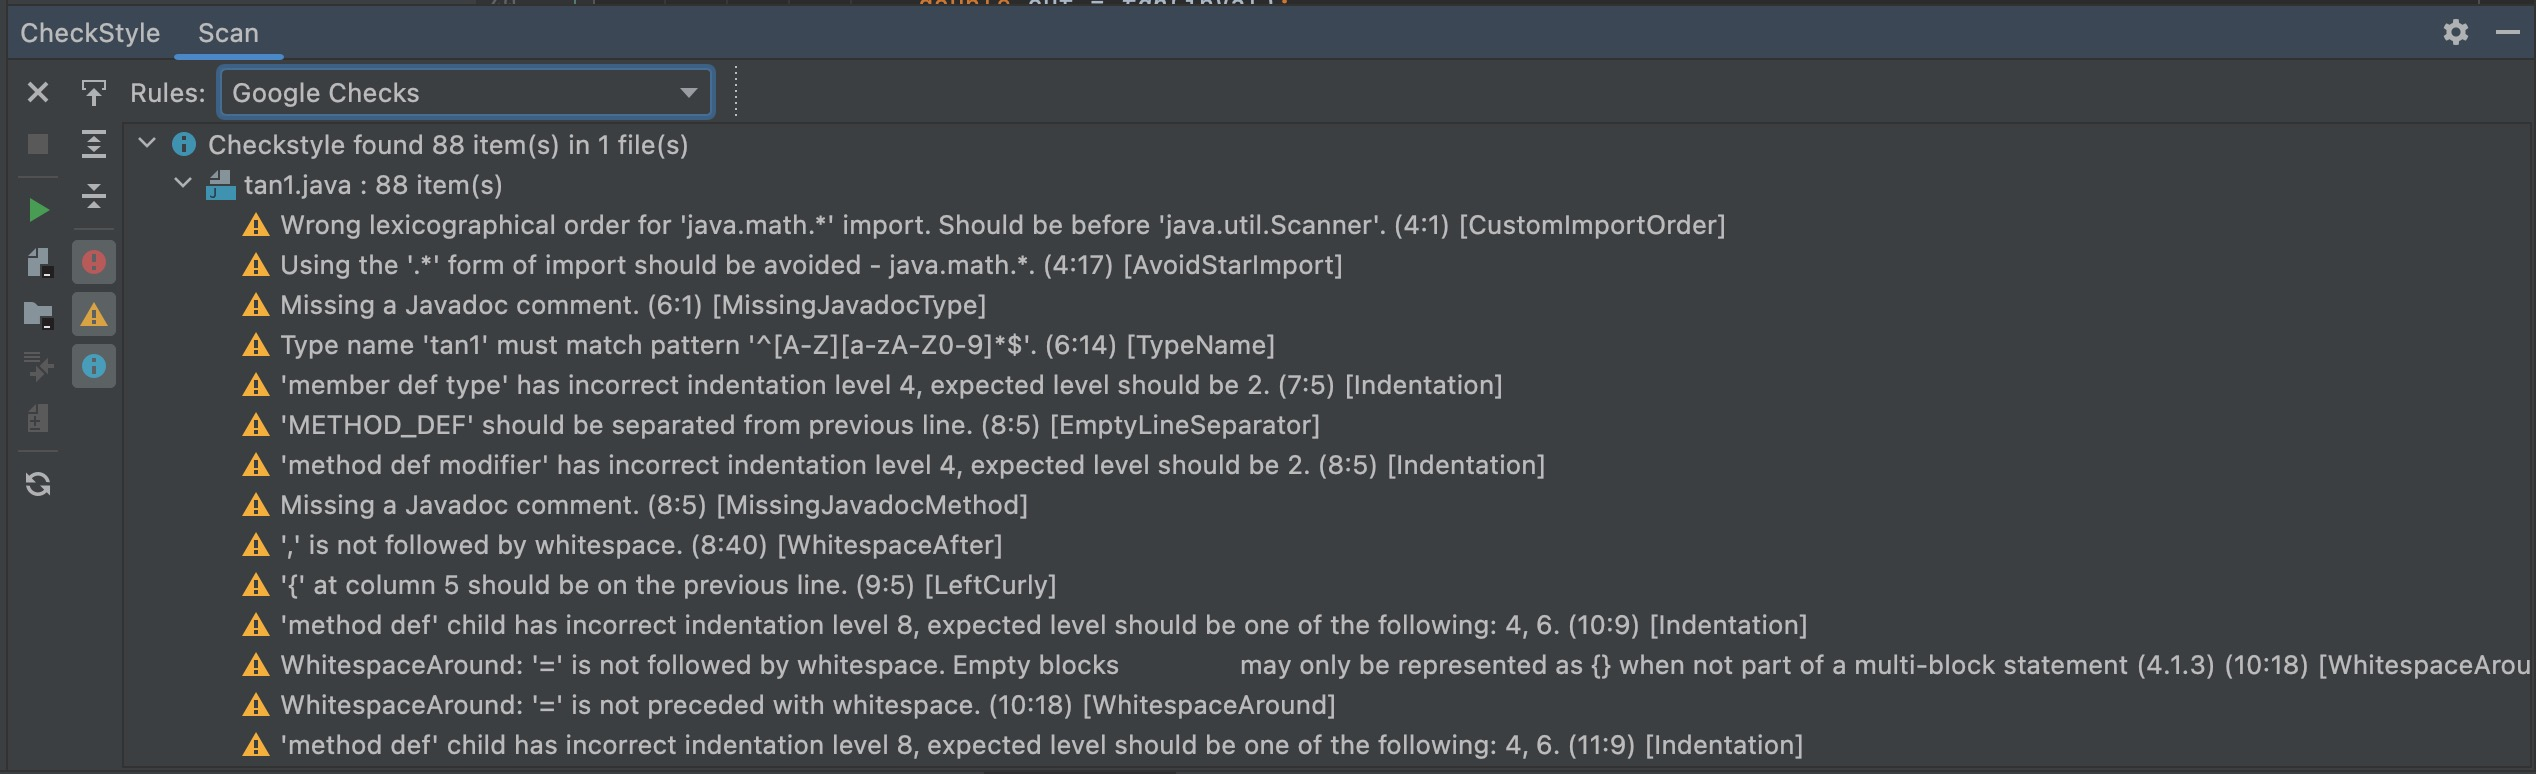
\includegraphics[scale=0.15]{Checkstyle.png}
\item
description: Checkstyle snapshot of my tan(x) function source code.
\item
advantages:Some information is useful for making my source code more easily readable. Like avoiding using ".*" form of import and add whitespace between variables and symbols.
\item
disadvantages: It lacks categories like "spaces", "indentation". Using categories can help the user identify his/her problems quickly.


%hier werd verwezen naar de tabel die als \label (naam} 'tabel1' kreeg.


%met enumerate genereer je een opsomming, itemize maakt verschillende puntjes
\begin{thebibliography}{99}  
\bibitem{ref1}Oracle, Code Conventions for the Java TM Programming Language, https://www.oracle.com/java/technologies/javase/codeconventions-contents.html, 1999.  
\end{thebibliography}
\end{document}
